\documentclass[unicode,11pt,a4paper,oneside,numbers=endperiod,openany]{scrartcl}

% Required package
\usepackage{amssymb}
\usepackage{graphicx}
\usepackage{amsmath}
\usepackage{matlab-prettifier}
\usepackage{float}
\usepackage[export]{adjustbox}
\usepackage{multirow}

\renewcommand{\thesubsection}{\arabic{subsection}}

% vector shortcut
\newcommand{\myv}{\mathbf}

\input{assignment.sty}
\begin{document}


\setassignment
\setduedate{Wednesday, 11 October 2023, 23:59 AM}

\serieheader
{Numerical Computing}
{2023}
{\textbf{Student:} Jeferson Morales Mariciano \\\\}
{\textbf{Discussed with:} Michele Dalle Rive, Filippo Piloni, Leonardo Birindelli}
{Solution for Project 1}{}
\newline

\assignmentpolicy

\newpage

% EXERCISE 1 %%%%%%%%%%%%%%%%%%%%%%%%%%%%%%%%%%%%%%%%%%%%%%%%%%%%%%%%%%%%%%%%%%%%%%%%%%%%%%%%%%%%%%
\subsection{Theoretical questions [15 points]}

\begin{enumerate}
    \item[(a)] \textbf{What are an eigenvector, an eigenvalue and an eigenbasis?}

        From Linear Algebra course notes: \\
        Let vector space $V$ and $A: V \rightarrow V$ be a linear mapping of $V$ into itself. \\
        Vector $\vec{v} \in V, \vec{v} \neq \vec{0}$ is \textbf{eigenvector} of matrix $A$ if $\exists$ scalar
        $\lambda: A\vec{v} = \lambda\vec{v}$. \\
        Hence, a non-zero vector remaining in the same direction after the application of a linear transformation A.

        Scalar $\lambda$ is an \textbf{eigenvalue} scaling factor of $A$ belonging to eigenvector $\vec{v}$. \\
        It represents the multiplying factor by which the correspondent eigenvector is compressed or stretched when a linear transformation matrix $A$ is applied, quantifying how a particular vector changes in magnitude. \\
        It respects $A\vec{v}=\lambda\vec{v}$.\\
        Eigenvalues and eigenvectors are also called characteristic values and vectors.

        An \textbf{eigenbasis} is a basis in which every vector is an eigenvector meaning the set of linearly independent eigenvectors of a square matrix $A$ that spans the entire vector space $V$ associated with such matrix.


    \item[(b)] \textbf{What assumptions should be made to guarantee convergence of the power method?}

        From book sections:

        \begin{itemize}
            \item "8.1  The power method and variants":
                  \begin{itemize}
                      \item
                            Tend towards the direction of the dominant eigenvector.

                      \item
                            for the Page Rank problem regarding the computation of the dominant eigenvector of a large and very sparse matrix,
                            the problem has a unique real solution x and the matrix:
                            \begin{itemize}
                                \item has an eigenvalue 1
                                \item such eigenvalue is also the dominant eigenvalue
                                \item algebraic multiplicity 1
                            \end{itemize}
                  \end{itemize}

            \item "Developing the power method"
                  \begin{itemize}
                      \item
                            Iterate magnitude check: repeating the normalization of $\vec{v_k}$ at each iteration to prevent accelerating roundoff error growth.

                      \item
                            Exclude possibility of equality of magnitudes: assuming eigenvalues $\lambda_1$, $\lambda_2$, ..., $\lambda_n$ are sorted in decreasing
                            order in terms of magnitude and the magnitude of the second eigenvalue is smaller than that of the first.
                  \end{itemize}

            \item "Example 8.3"
                  \begin{itemize}
                      \item
                            Dangling node correction: populate columns of nodes with no outlinks from values
                            already set to 0 to $\frac{1}{n}$ where $n$ is the number of total nodes.

                      \item
                            Strong component with cycle path correction: ensure random jump every finite number of steps.
                            Typically $p \in [0.8, 0.9]$, so jump every 5 steps on avg.
                  \end{itemize}

            \item "Assessing limitations of the power method"
                  \begin{itemize}
                      \item
                            exclude defective matrices: all eigenvectors of the matrix are linearly independent and span $\mathbb{R}^n$.
                            Requirement since notion of \textit{geometric multiplicity of eigenvalues} states
                            that power method becomes painfully slow.
                            Worse than ratios of dominant eigenvalues.

                      \item
                            requiring $\beta_1 \neq 0$ in  $\vec{v_0}$ initial guess in iteration so $\vec{v_0}$ has a component in the direction of $\vec{x_1}$. Low restriction.
                            Even if $\beta_1 = 0$, roundoff errors in the computation introduce a small component in all eigenvector directions, leveraging the error.

                      \item
                            reasonable minimal distance between $\lambda_2$ and $\lambda_1$.
                            Given power method asymptotic error constant is $|\frac{\lambda_1}{\lambda_2}|$,
                            if $\lambda_2$ is very close in magnitude to $\lambda_1$, convergence is extremely slow.
                  \end{itemize}
        \end{itemize}

    \item[(c)] \textbf{What is the shift and invert approach?}

        From "Shift and invert technique" book section: \\
        The inverse iteration guarantees faster convergence that power method at the considerable price of having to solve a linear system in each iteration.
        It overcomes the extremely slow convergence of power method when $\lambda_1$ and $\lambda_2$ are close together. \\

        It uses the shift and inverse technique: \\
        If the eigenvalues of $A$ are $\lambda_j$, the eigenvalues of $A - \alpha I$ are $\lambda_j - \alpha$,
        and the eigenvalues of $B = (A - \alpha I)^{-1}$ are $\mu_j = \frac{1}{\lambda_j - \alpha}$.

        So by applying the power method to $B$ and supposing $\lambda_2$ is the eigenvalue of $A$ closes to $\lambda_1$,
        then such iteration still converges linearly but at rate $|\frac{\mu_2}{\mu_1}| = |\frac{\lambda_1 - \alpha}{\lambda_2 - \alpha}|$.

        If $\alpha$ is very close to $\lambda_1$, convergence is expected to be very fast.
        To choose the parameter $\alpha$ close to $\lambda_1$ use the \textit{Rayleigh quotient} which is a good approximation to an eigenvalue for a given vector.
        So the shift of $\alpha$ is dynamic and convergence order reaches cubic complexity.


    \item[(d)] \textbf{What is the difference in cost of a single iteration of the power method, compared to the inverse iteration?}

        From "Shift and invert technique" book section: \\

        Computational cost: in the power method, each iteration involves a matrix-vector product with $O(n^2)$,
        while the inverse iteration requires at each loop to solve a linear system with $O(n^3)$. \\

        Use cases: for inverse iteration it can happen to entertain methods that require thousands of matrix-vector multiplications
        for one iteration of the inverse iteration.
        Thus, convergence may be very fast for it to be effective, and tackling huge examples is out of question
        like Internet searching.
        Inverse iteration is attractive for smaller problems or ones with special structure that enable fast direct methods.


    \item[(e)] \textbf{What is a Rayleigh quotient and how can it be used for eigenvalue computations?}

        From A First course in Numerical Computing - Developing the power method: \\
        The Reyligh quotient defined for any vector and denoted by \\

        \begin{equation} \label{rayleigh quotient}
            \mu(\textbf{v}) = \frac
            {\textbf{v}^T A\textbf{v}}
            {\textbf{v}^T \textbf{v}}
        \end{equation}

        is the closest possible approximation to an eigenvalue. \\
        It is used in the Shift and Inverse technique to find eigenvalues and reach a cubic convergence complexity
        since the $\alpha$ factor changes dynamically at each iteration even though it is computationally expensive:
        it requires matrix refactoring at each iteration.

\end{enumerate}
\cleardoublepage

% EXERCISE 2 %%%%%%%%%%%%%%%%%%%%%%%%%%%%%%%%%%%%%%%%%%%%%%%%%%%%%%%%%%%%%%%%%%%%%%%%%%%%%%%%%%%%%%
\subsection{Connectivity matrix and subcliques [5 points]}
The connectivity matrix for the ETH500 data set (ETH500.mat) has various small, almost entirely nonzero, submatrices that produce dense patches near the diagonal of the spy plot.
You can use the zoom button to find their indices.
The first submatrix has, e.g., indices around 80. Mathematically, a graph where all nodes are connected to each other
is known as a clique. Identify the organizations within the ETH community that are responsible for these near cliques. \\

\begin{figure}[h!]
    \centering
    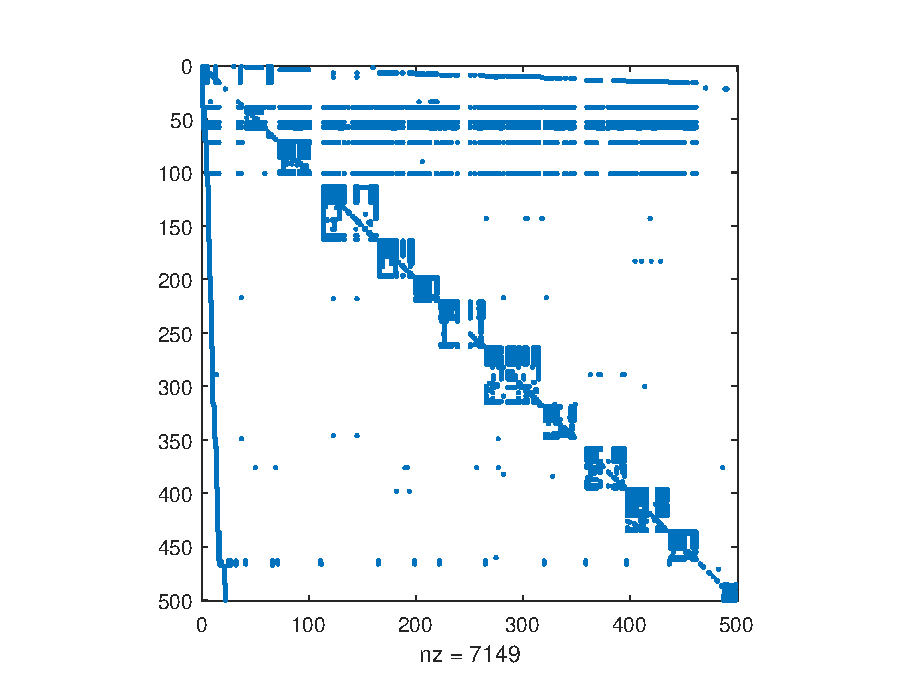
\includegraphics[width=0.7\textwidth]{figures/cliques.eps}
    \caption{connectivity matrix for ETH500}
    \label{fig:cliques}
\end{figure}

Table \ref{table:cliques} shows ETH community organizations URL and name responsible to form the cliques around the diagonal of the spy plot.
Cliques top-left and bottom-right coordinates are provided to identify the organizations in the plot.

\begin{table}[h!]
    \centering
    \begin{tabular}{||p{2.7in} c c c||}
        \hline
        Name & Domain                                       & CoordTopLeft & CoordBottomRight \\ [0.5ex]
        \hline\hline
        Dept. of Civil, Environmental and Geomatic Engineering
             & \href{http://www.biol.ethz.ch}{biol.ethz.ch}
             & (73, 71)                                     & (86, 86)                        \\

        Department of Materials
             & \href{https://mat.ethz.ch}{mat.ethz.ch}
             & (116, 113)                                   & (129, 128)                      \\

        Department of Mechanical and Process Engineering
             & \href{https://mavt.ethz.ch}{mavt.ethz.ch}
             & (166, 164)                                   & (178, 178)                      \\

        Department of Biology
             & \href{https://biol.ethz.ch}{biol.ethz.ch}
             & (200, 198)                                   & (213, 213)                      \\

        Department of Chemistry and Applied Biosciences
             & \href{https://chab.ethz.ch}{chab.ethz.ch}
             & (224, 221)                                   & (233, 236)                      \\

        Department of Mathematics
             & \href{http://www.math.ethz.ch}{math.ethz.ch}
             & (266, 264)                                   & (278, 279)                      \\

        Department of Earth Sciences
             & \href{http://www.erdw.ethz.ch}{erdw.ethz.ch}
             & (321, 319)                                   & (328, 332)                      \\

        Department of Environmental Systems Science
             & \href{http://www.usys.ethz.ch}{usys.ethz.ch}
             & (360, 358)                                   & (369, 370)                      \\

        Department of Management, Technology, and Economics
             & \href{https://mtec.ethz.ch/}{mtec.ethz.ch}
             & (398, 396)                                   & (406, 407)                      \\

        Department of Humanities, Social and Political Sciences
             & \href{http://www.gess.ethz.ch}{gess.ethz.ch}
             & (438, 436)                                   & (451, 451)                      \\ [1ex]
        \hline
    \end{tabular}
    \caption{Cliques formed by ETH community organizations}
    \label{table:cliques}
\end{table}
\cleardoublepage

% EXERCISE 3 %%%%%%%%%%%%%%%%%%%%%%%%%%%%%%%%%%%%%%%%%%%%%%%%%%%%%%%%%%%%%%%%%%%%%%%%%%%%%%%%%%%%%%
\subsection{Connectivity matrix and disjoint subgraphs [10 points]}

\begin{figure}[H]
    \centering
    \includegraphics[width=0.3\textwidth]{figures/graph_disjoint}
    \caption{graph of six-node subset of the Web}
    \label{fig:graph_disjoint}
\end{figure}

Given the Figure \ref{fig:graph_disjoint} graph of six node subset of the web containing 2 disjoint subgraphs: \\

\begin{enumerate}
    \item \textbf{What is the connectivity matrix G? Which are its entries?}

          $n$ webpages and vertices $U \in \mathbb{R}^n$, $U = \begin{bmatrix} alpha & beta & gamma & delta & rho & sigma \end{bmatrix}^\intercal$ are given.

          The connectivity matrix $G \in \mathbb{R}^{n \times n}$ is a sparse logical non-symmetric matrix where $n$ is the number of web pages from $U$, corresponding to link structure of a directed graph. \\
          For any $j$ page: the $j$th column corresponds the outlinks from page $j$;
          while the $j$th row indicate its inlinks.

          The entries of $G$ for Figure \ref{fig:graph_disjoint} are:

          \begin{math}
              G =
              \begin{bmatrix}
                  0 & 0 & 0 & 1 & 0 & 0 \\
                  1 & 0 & 0 & 0 & 0 & 0 \\
                  1 & 1 & 0 & 0 & 0 & 0 \\
                  0 & 1 & 1 & 0 & 0 & 0 \\
                  0 & 0 & 0 & 0 & 0 & 1 \\
                  0 & 0 & 0 & 0 & 1 & 0 \\
              \end{bmatrix}
          \end{math}

    \item \textbf{What are the PageRanks if the hyperlink transition probability p assumes the default value of 0.85?}

          Model and executing Pagerank algorithm in Matlab to ease arguments for answers:

          \begin{lstlisting}[
            frame=single,
            numbers=left,
            style=Matlab-editor,
            basicstyle=\mlttfamily\small,
            caption={Exercise Matlab model},
            captionpos=b]
U = ["alpha", "beta", "gamma", "delta", "rho", "sigma"];
n = size(U, 2);
inlinks = [[1,4]; [2,1]; [3,1]; [3,2]; [4,2]; [4,3]; [5,6]; [6,5]]; 
G = sparse(inlinks(:,1), inlinks(:,2), ones(1, size(inlinks, 1)));
p = .85;
pagerank(U, G, p);  % function pagerank provided with assignment
        \end{lstlisting}

          \begin{figure}[H]
              \centering
              \includegraphics[width=0.7\textwidth]{figures/ex3p2_pagerank}
              \caption{Pagerank values for $p = 0.85$}
              \label{fig:ex3_pagerank_histogram}
          \end{figure}

          \begin{table}[H]
              \centering
              \begin{tabular}{||c c c c c||}
                  \hline
                  Name  & Index & Inlinks & Outlinks & Pagerank          \\ [0.5ex]
                  \hline\hline
                  delta & 4     & 2       & 1        & 0.203693938456013 \\
                  alpha & 1     & 1       & 2        & 0.198139847687611 \\
                  rho   & 5     & 1       & 1        & 0.166666666666667 \\
                  sigma & 6     & 1       & 1        & 0.166666666666667 \\
                  gamma & 3     & 2       & 1        & 0.155623445255809 \\
                  beta  & 2     & 1       & 2        & 0.109209435267235 \\ [1ex]
                  \hline
              \end{tabular}
              \caption{Results for $p = 0.85$}
              \label{table:ex3_pagerank_table_p1}
          \end{table}

          Page \textbf{delta} is the highest page ranked. \\
          Inlinks and outlinks put to emphasize that $degree \neq pagerank$ of nodes.

    \item \textbf{Describe what happens with this example to both the definition of PageRank and the computation done by pagerank in the limit p → 1.}

          Update matlab code at line $5$:  $p = .9999999999$.


          \begin{figure}[H]
              \centering
              \includegraphics[width=0.7\textwidth]{figures/ex3p3_pagerank.eps}
              \caption{Pagerank values for $p = 0.9999999999$}
              \label{fig:ex3_pagerank_p2_histogram}
          \end{figure}

          \begin{table}[H]
              \centering
              \begin{tabular}{||c c c||}
                  \hline
                  Name  & Index & Pagerank          \\ [0.5ex]
                  \hline\hline
                  delta & 4     & 0.205128199377198 \\
                  alpha & 1     & 0.205128216388855 \\
                  rho   & 5     & 0.166666666666667 \\
                  sigma & 6     & 0.166666666666667 \\
                  gamma & 3     & 0.153846149558366 \\
                  beta  & 2     & 0.102564101342246 \\ [1ex]
                  \hline
              \end{tabular}
              \caption{Results for $p = 0.9999999999$}
              \label{table:ex3_pagerank_table_p2}
          \end{table}

          With $p = 0.85$, the random walker have strongly the concept of following links from nodes, nevertheless it randomly performs jumps to other graph nodes with $0.15$ chance. \\

          With $p \rightarrow 1$, the random walker tend to always respect the notion of following links by putting more weight to link graph, hence never jumping randomly to other nodes of the network.
          Inlinks and outlinks reach the maximum weight for determining Page Rank of pages.\\

          Whether or not having such high $p$ in both cases is \textit{"good"} is a purely modeling question:
          following dogmatically graph linking is not ensured to be optimal and values for damping parameter $p$ is still subject to debate.

\end{enumerate}

\cleardoublepage

% EXERCISE 4 %%%%%%%%%%%%%%%%%%%%%%%%%%%%%%%%%%%%%%%%%%%%%%%%%%%%%%%%%%%%%%%%%%%%%%%%%%%%%%%%%%%%%%
\subsection{PageRanks by solving a sparse linear system [25 points]}
The function \textit{pagerank(U,G)} computes PageRanks by solving a sparse linear system. It then plots a bar graph and prints the dominant URLs.

\subsubsection{Create \textit{pagerank1.m} by modifying \textit{pagerank.m} to use the power method instead of solving the sparse linear system.}

An appropriate test to terminate the power iteration is
to set a threshold \textit{epsilon} to be always lower than
the taxicab norm of the difference between the current and previous rank vector. \\
Precision has been set to $1e-7$.

\subsubsection{Create \textit{pagerank2.m} by modifying \textit{pagerank.m} to use the inverse iteration.
    Use your functions \textit{pagerank1.m} and \textit{pagerank2.m} (set $\alpha = 0.99$)
    to compute the PageRanks of the six-node example presented in Figure \ref{fig:ex4-graph}.
    Make sure you get the same result from each of your three functions.}

\begin{figure}[H]
    \centering
    \includegraphics[width=0.3\textwidth]{figures/ex4_graph}
    \caption{Tiny web graph}
    \label{fig:ex4-graph}
\end{figure}

Comparing results from power method and inverse iteration method with $precision = 1e-7$:

\begin{table}[H]
    \centering
    \begin{tabular}{||c c c c c||}
        \hline
        Name  & Index & Default Implementation & Power Method      & Inverse Iteration \\ [0.5ex]
        \hline\hline
        alpha & 1     & 0.321016940895182      & 0.321016945146995 & 0.321016939512291 \\
        sigma & 6     & 0.200743999937897      & 0.200743995967436 & 0.200743998918274 \\
        beta  & 2     & 0.170543038221924      & 0.170543035357689 & 0.170543036970788 \\
        delta & 4     & 0.136792591301763      & 0.136792592485608 & 0.136792591830432 \\
        gamma & 3     & 0.106591629585789      & 0.106591631875861 & 0.106591629882945 \\
        rho   & 5     & 0.064311800057445      & 0.064311799166412 & 0.064311802885270 \\ [1ex]
        \hline
    \end{tabular}
    \caption{Pagerank results for $p = 0.85$}
    \label{table:ex4p2_pagerank_table}
\end{table}

\begin{table}[H]
    \centering
    \begin{tabular}{||c c c||}
        \hline
        /                 & Time avg   & Iterations \\ [0.5ex]
        \hline\hline
        Default Time      & 7.2890e-05 & -          \\
        Power Method      & 8.0340e-05 & 29         \\
        Inverse Iteration & 1.0034e-04 & 4          \\ [1ex]
        \hline
    \end{tabular}
    \caption{Pagerank method comparison}
    \label{tab:ex4p2_comparison}
\end{table}

Timing average values given by \textit{timeit(f)} function in Matlab. \\
The first $5$ digits show the same result for all the three methods. \\
The inverse method is observed to be the one taking most, such behavior can be explained by remembering that
the cost of solving a linear equation is $O(n^3)$ for each iteration. \\
Remember that generally a cycle of the inverse iteration method correspond to $~$ hundreds
of cycle of the power method: the difference by magnitude.

\subsubsection{We now want to analyse the impact of $\alpha$ on the inverse iteration.
    Using the ETH500 example, set $\alpha$ equal to 0.8, 0.9, 0.95 and 1.
    Comment on the different number of iterations the four cases take until convergence.
    Analyse your results and explain what you observe.
    Hint: Check your solution x for all 4 cases. Are they always the same?}

With $p = 0.85$:

\begin{itemize}
    \item $\alpha = 0.8$ \\
          Negative values for pagerank are resulting from such plot and having negative value is not meaningful for the
          pagerank.
          In this case, $\alpha$ is such that the nearest eigenvector is the one with negative and positive values as displayed in the plot. \\
          $Iterations = 5.$

          \begin{figure}[H]
              \centering
              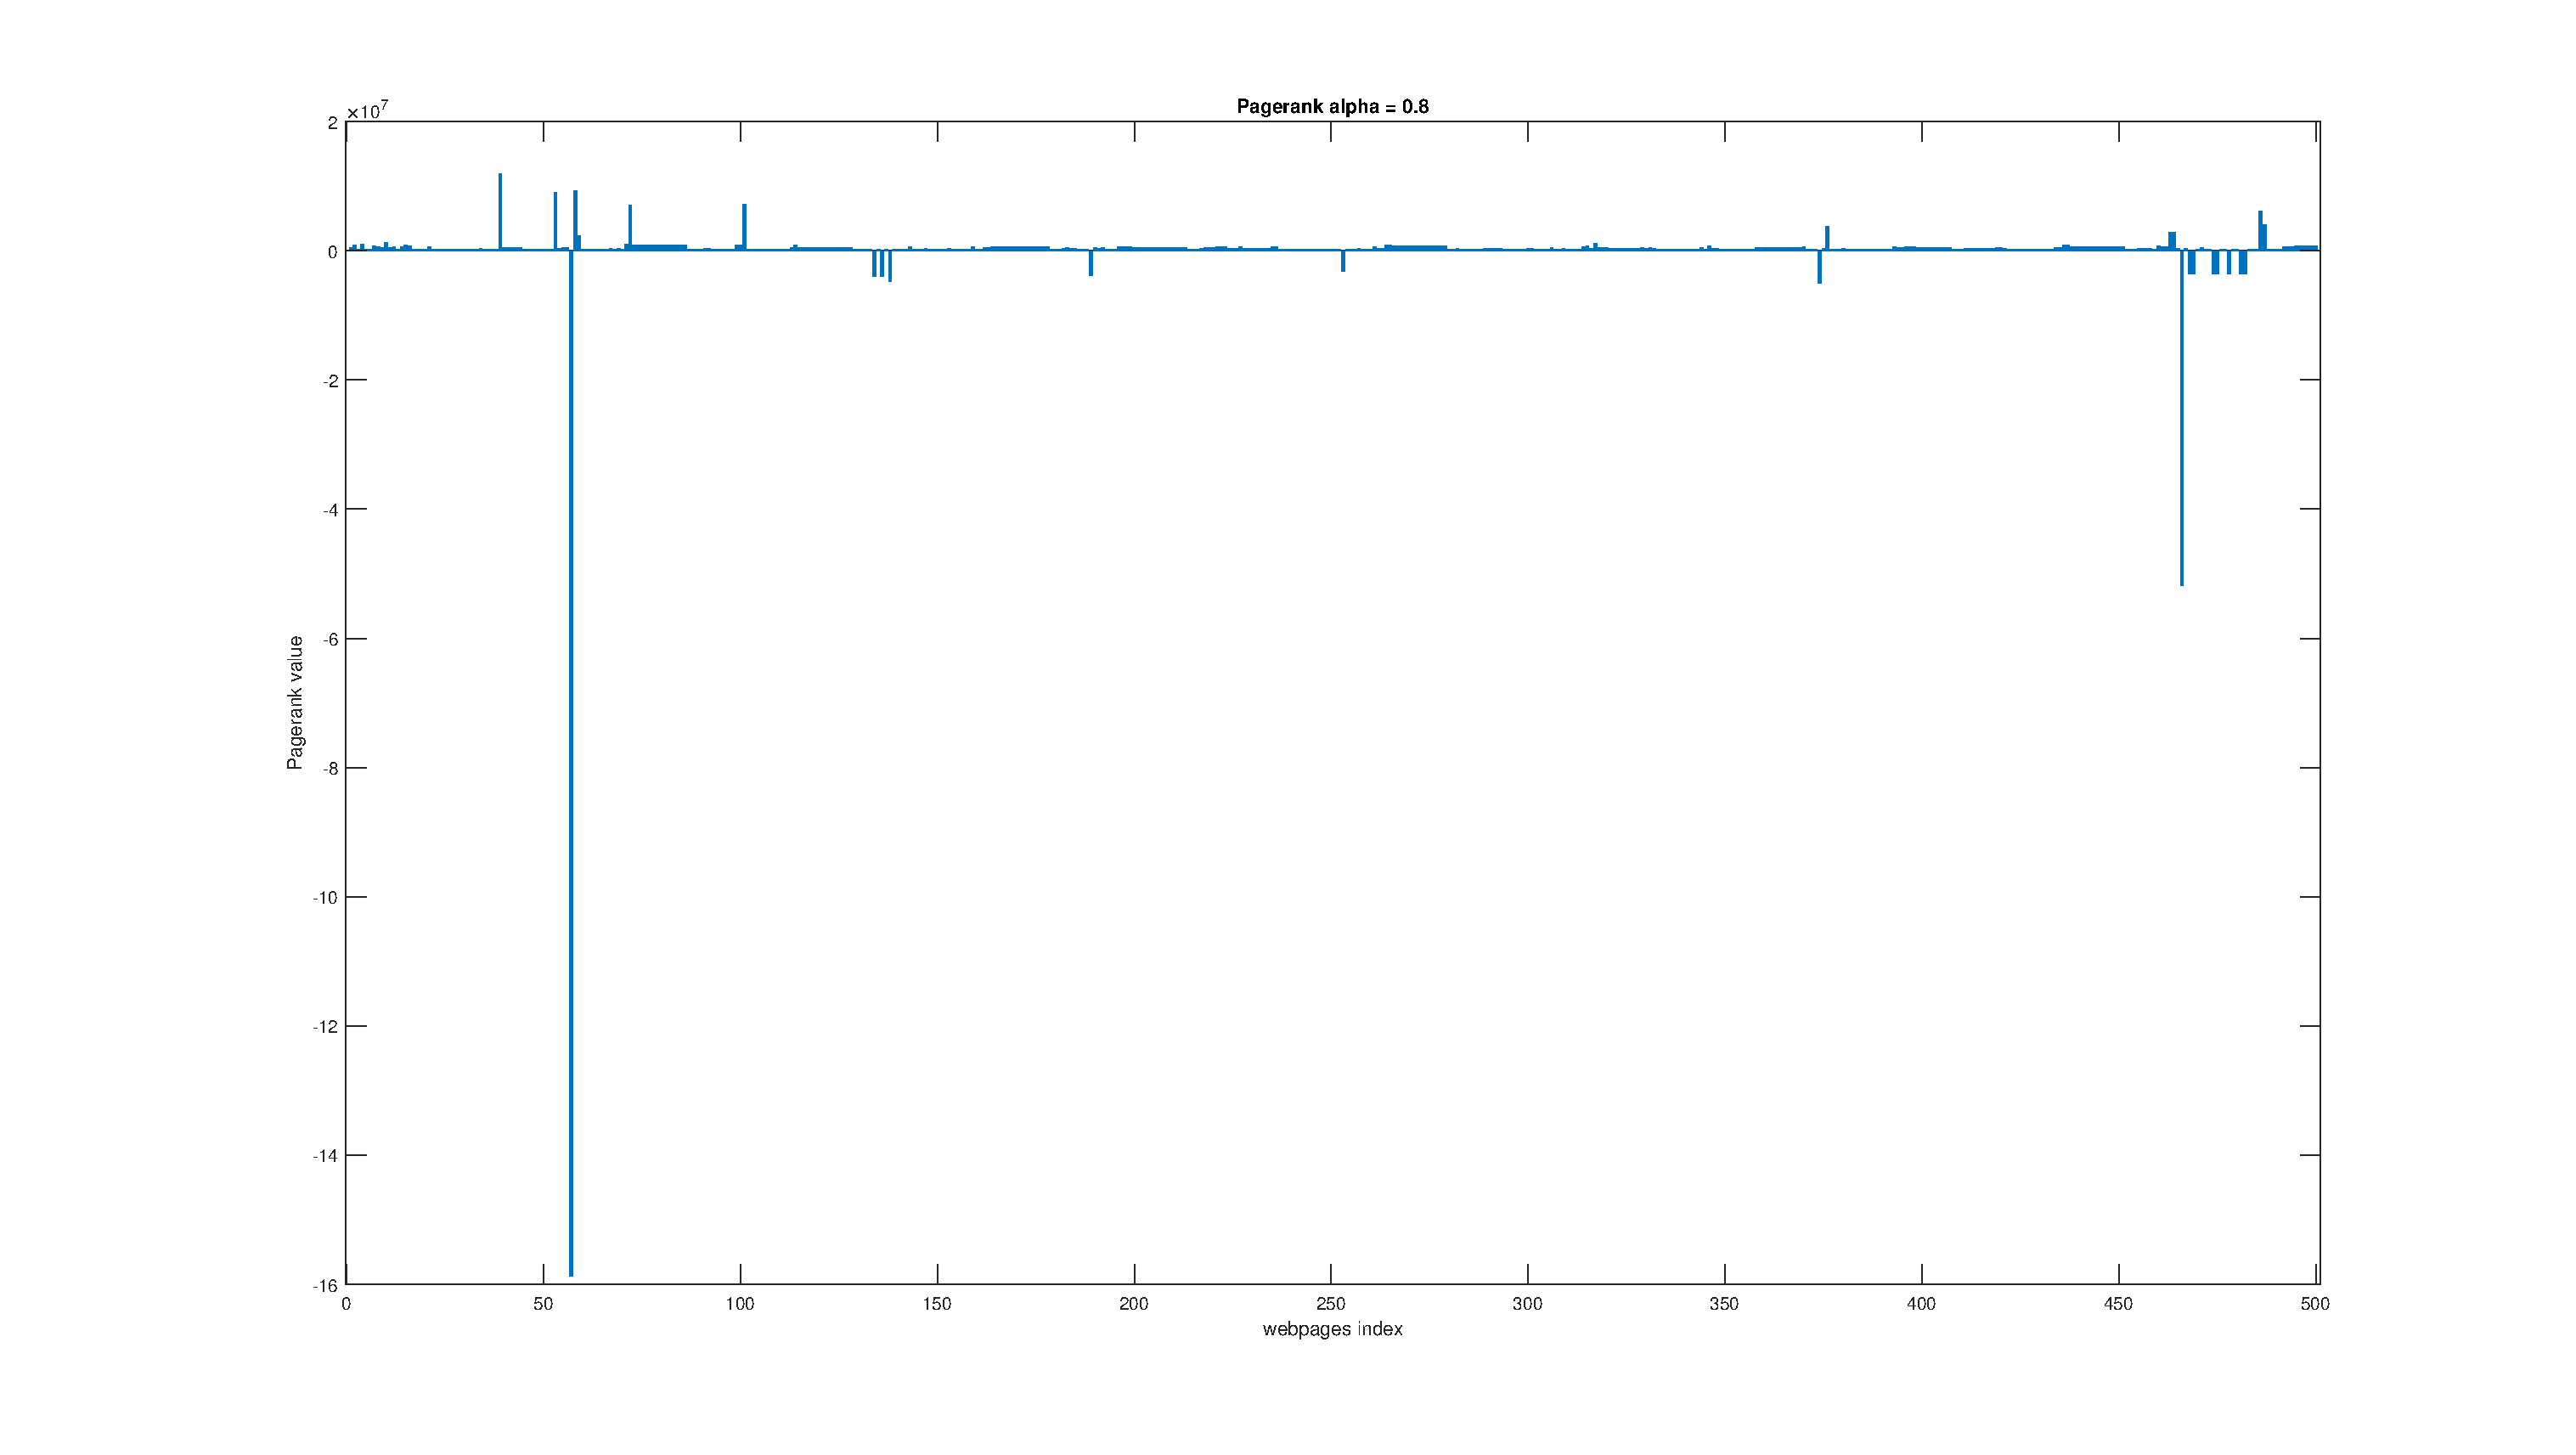
\includegraphics[width=1\textwidth, trim={0 0 0 0}]{figures/ex4p3_a08.eps}
              \caption{Iterative method for $\alpha = 0.8$}
              \label{fig:e4p3_a08}
          \end{figure}

    \item $\alpha = 0.9$ \\
          Instability: an infinite loop is caused by $\alpha$ since its value is making the matrix $B$ singular
          hence not invertible:
          it is not feasable to calculate the linear equation satisfying the inverse iteration exit condition
          and thus it does not converge. \\
          $Iterations = 100$, broke out of loop due to limit iterations threshold reached.

          \begin{figure}[H]
              \centering
              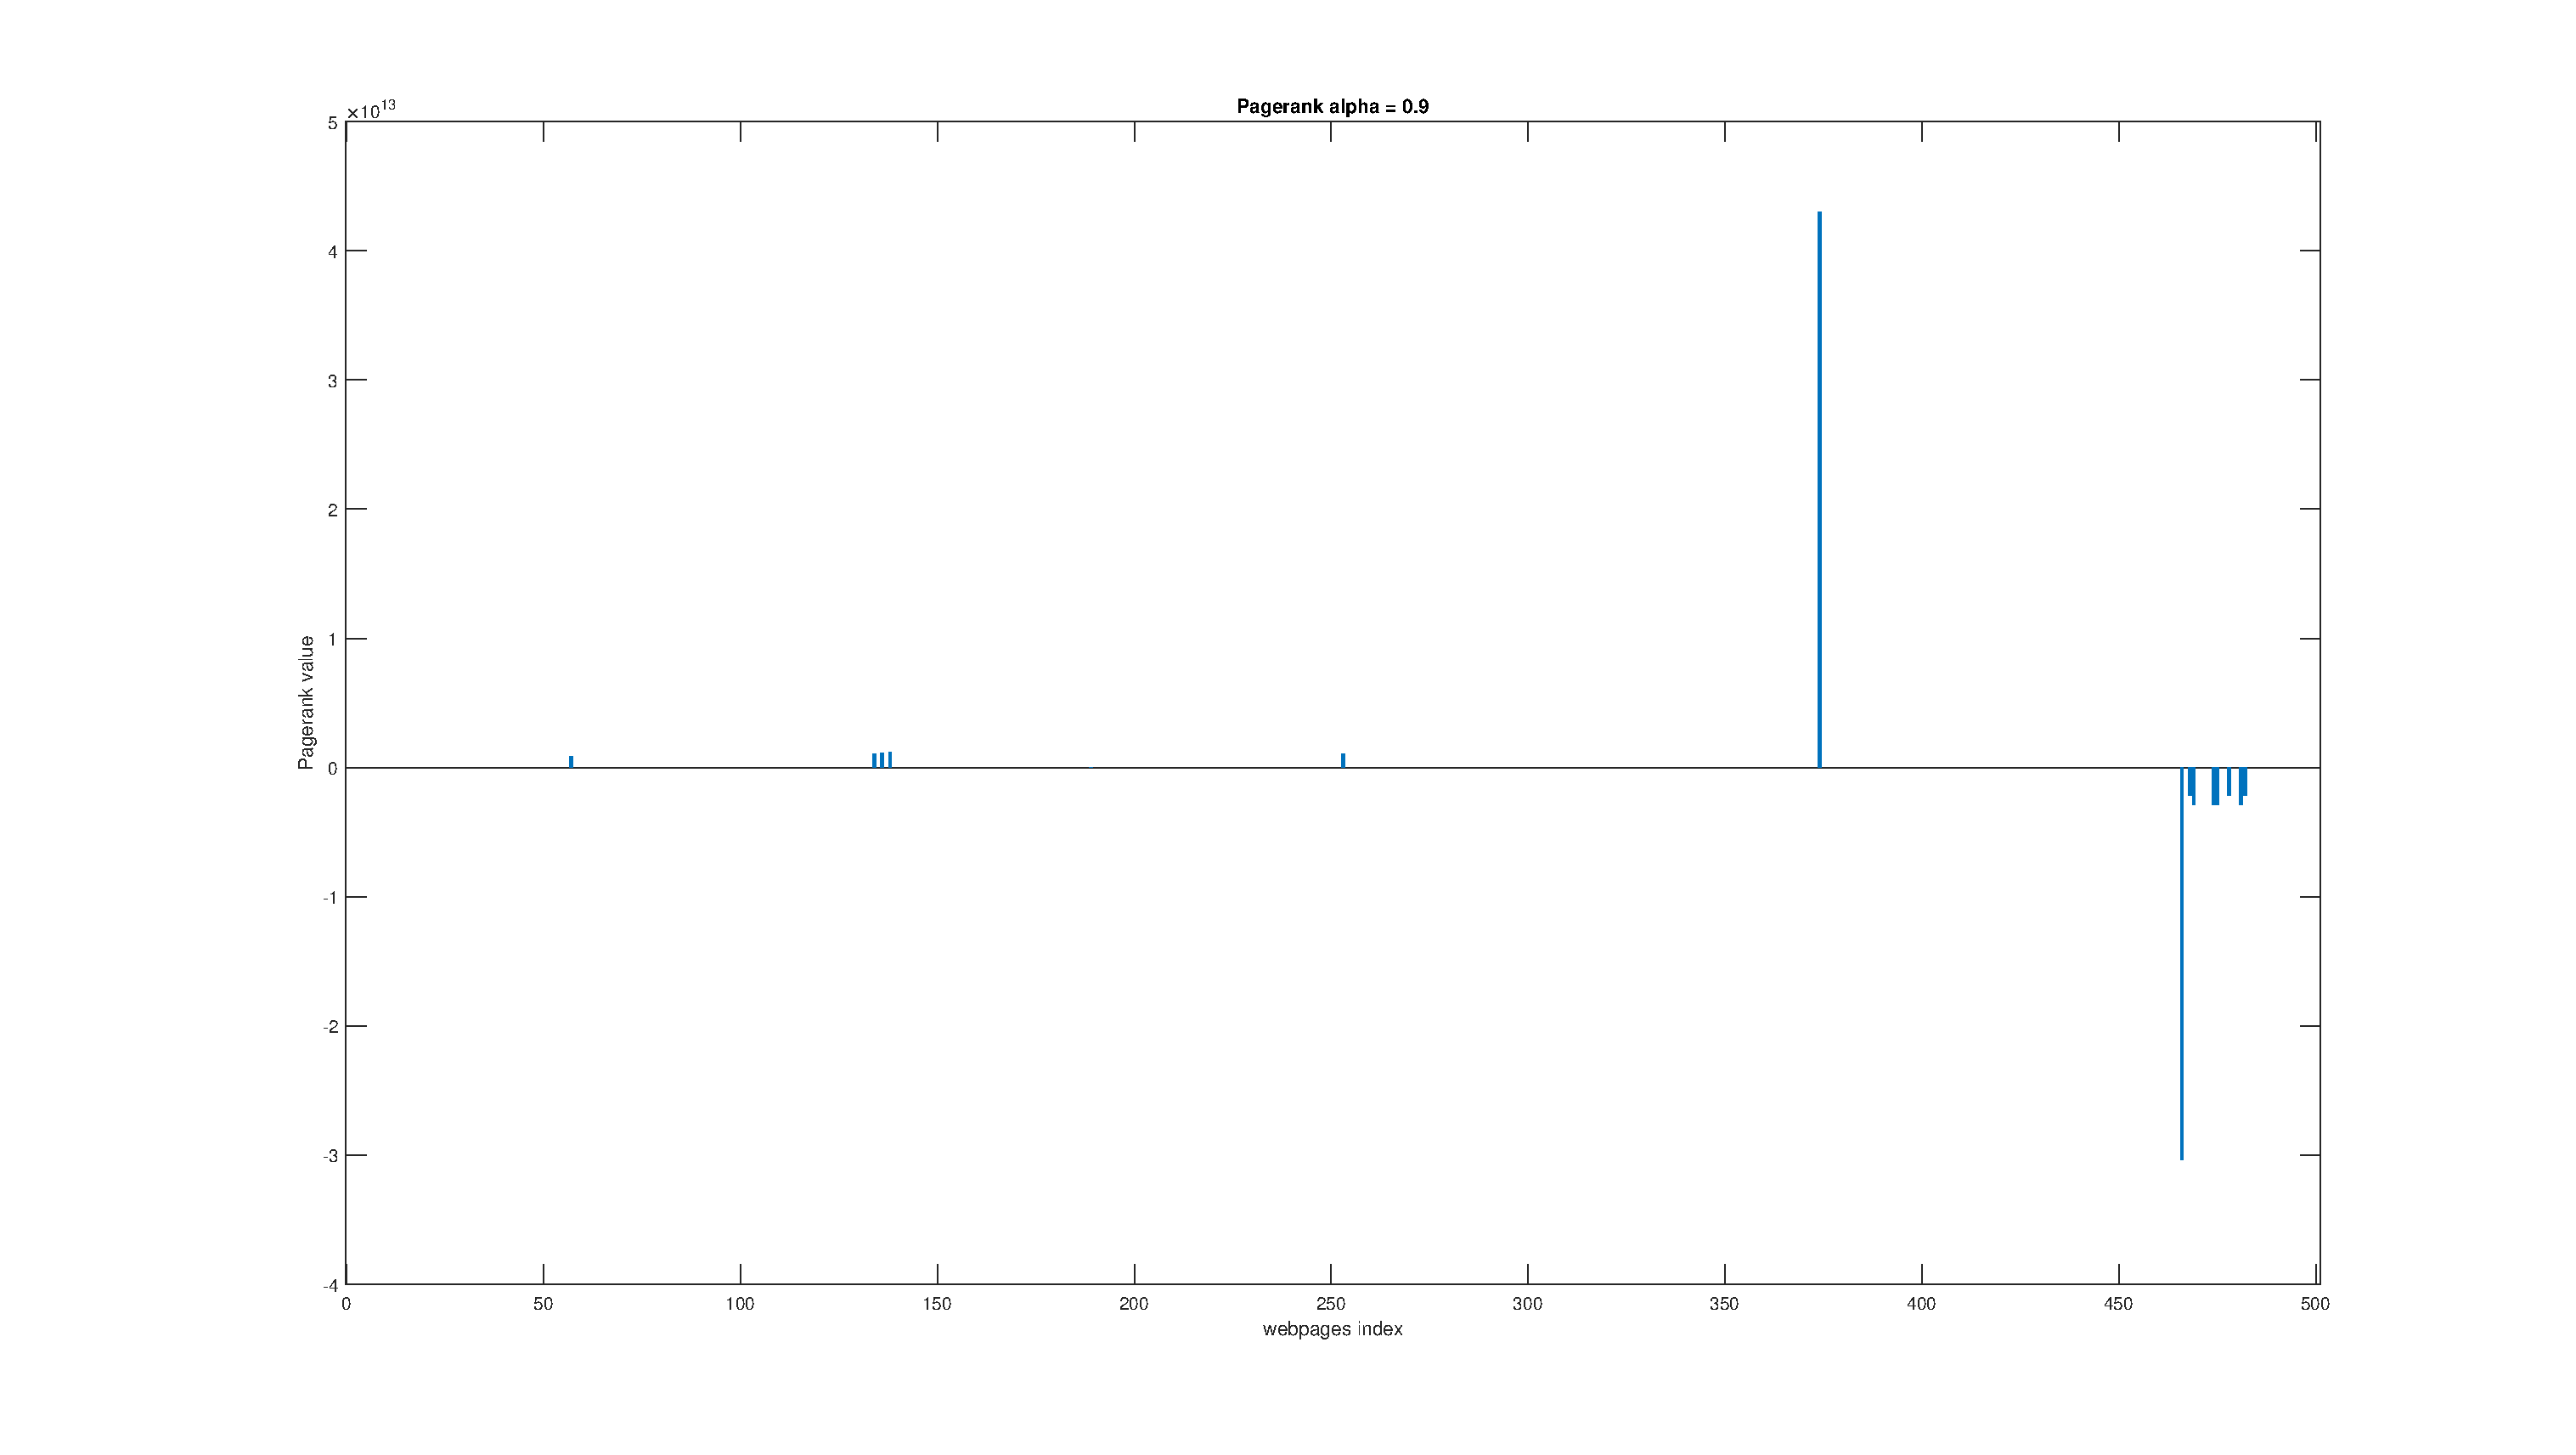
\includegraphics[width=1\textwidth, trim={0 0 0 0}]{figures/ex4p3_a09.eps}
              \caption{Iterative method for $\alpha = 0.9$ after $100$ iterations}
              \label{fig:e4p3_a09}
          \end{figure}

    \item $\alpha = 0.95$ \\
          The computation converges and the following result is plotted. \\
          $Iterations = 14.$

          \begin{figure}[H]
              \centering
              \includegraphics[width=1\textwidth, trim={0 0 0 0}]{figures/ex4p3_a095.eps}
              \caption{Iterative method for $\alpha = 0.95$}
              \label{fig:e4p3_a095}
          \end{figure}

    \item $\alpha = 1$ \\
          Instability: again an infinite loop caused by $\alpha$. \\
          Matrix $B$ is badly conditioned since its reciprocal condition number is near $0$:
          after building matrix $B = A - \alpha I$, check $rcond(B) < \epsilon \approx 0$. \\
          Perturbe $\alpha$ by a neglectible value for the machine precision to be able to to make it converge
          but the direction is a guess and results could be inaccurate.
          Matlab Message warning sent to the console:

          \textit{Warning: Matrix is close to singular or badly scaled. Results may be inaccurate. \\
              RCOND =  2.039751e-18.}

          Tweaking: after evaluating true the condition $\alpha < \epsilon = 1e-16$,
          perturbed $\alpha = \alpha - 1e-3$, recomputed $B$ whose new \textit{RCOND} is $0.000005$
          and forced convergence.
          $Iterations = 3.$

          \begin{figure}[H]
              \centering
              \includegraphics[width=1\textwidth, trim={0 0 0 0}]{figures/ex4p3_a1.eps}
              \caption{Iterative method for $\alpha = 1$}
              \label{fig:e4p3_a1}
          \end{figure}

          Or after forcing loop breaking given a threshold number of iterations set to $100$.

          \begin{figure}[H]
              \centering
              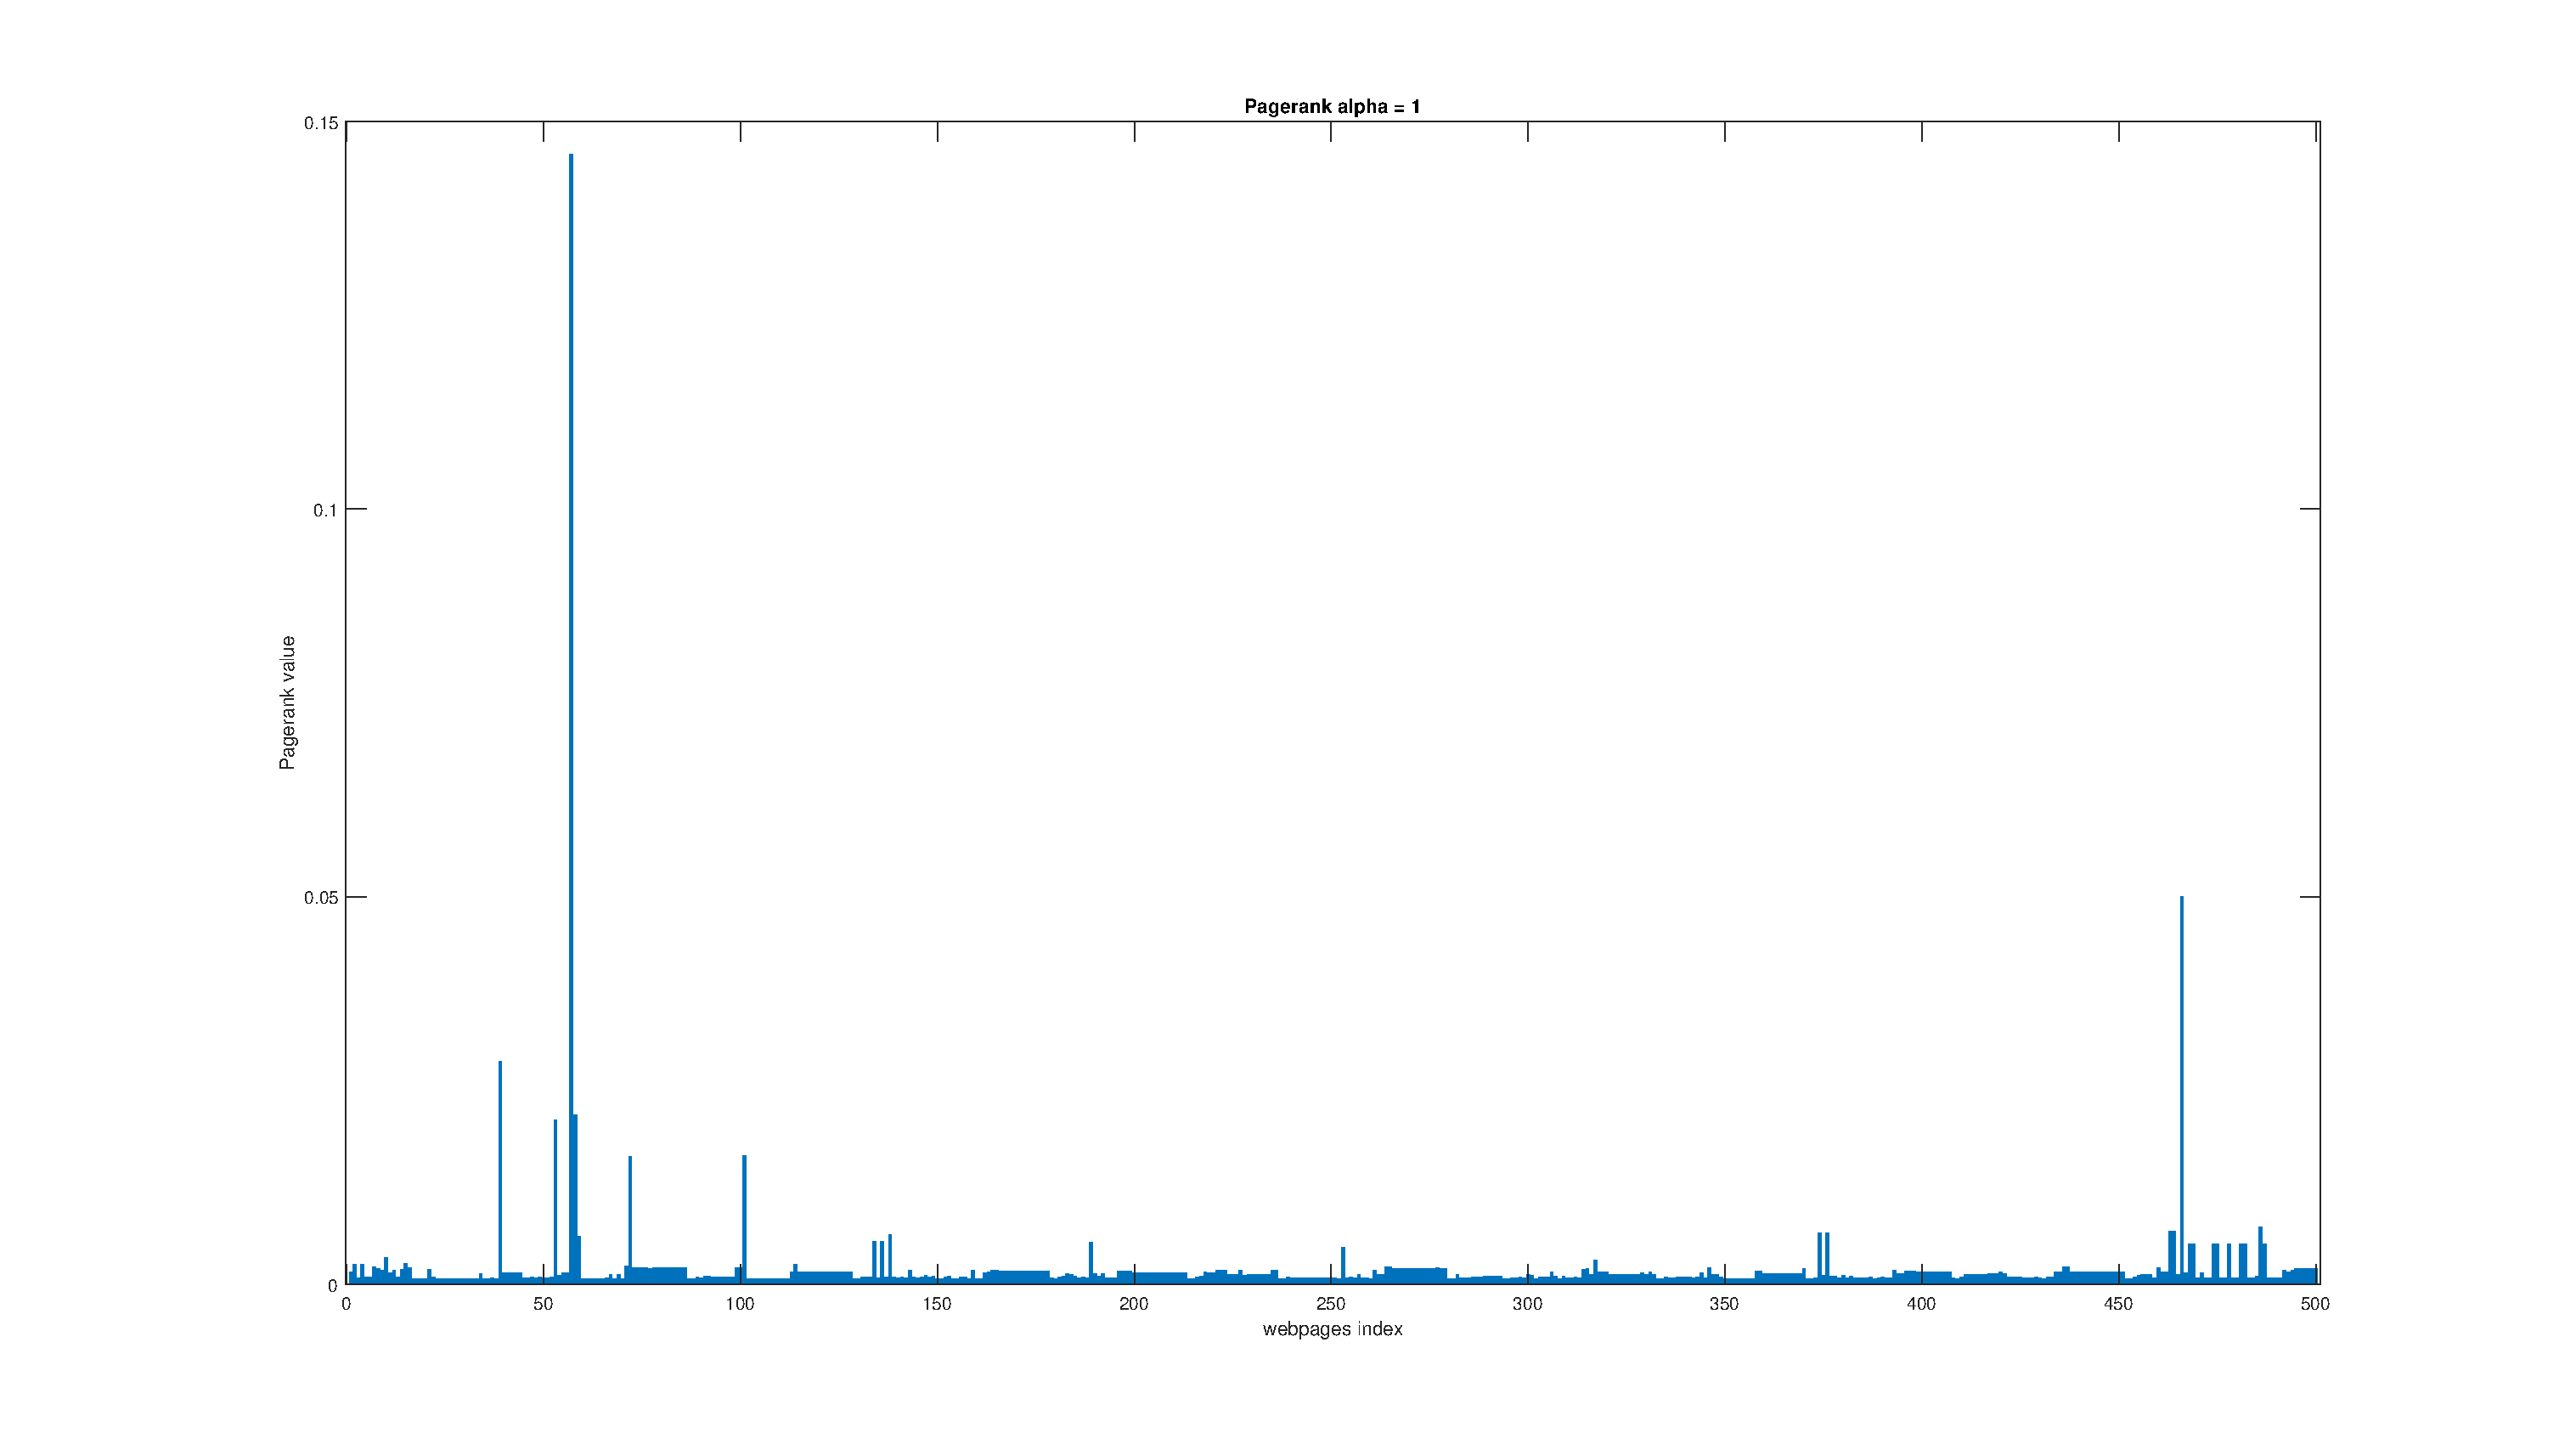
\includegraphics[width=1\textwidth, trim={0 0 0 0}]{figures/ex4p3_a1_maxit.eps}
              \caption{Iterative method for $\alpha = 1$ after $100$ iterations}
              \label{fig:e4p3_a1_maxit}
          \end{figure}

          Hence $x$ pagerank vector values are not always the same: despite the graph to analyze remaining the same,
          the value of $\alpha$ changes convergence direction to nearest eigenvector generating interesting behaviors
          analyzed above for the requested values.

\end{itemize}

\subsubsection{Use your functions \textit{pagerank1.m} and \textit{pagerank2.m} (set $\alpha = 0.99$) to compute the PageRanks of three selected graphs (\textit{web1.mat}, \textit{web2.mat} and \textit{web3.mat}).
    Report on the convergence of the two methods for these subgraphs and summarize the advantages and disadvantages
    of the power method implemented in \textit{pagerank1.m} against the inverse iteration in \textit{pagerank2.m}.}

\begin{figure}[H]
    \centering
    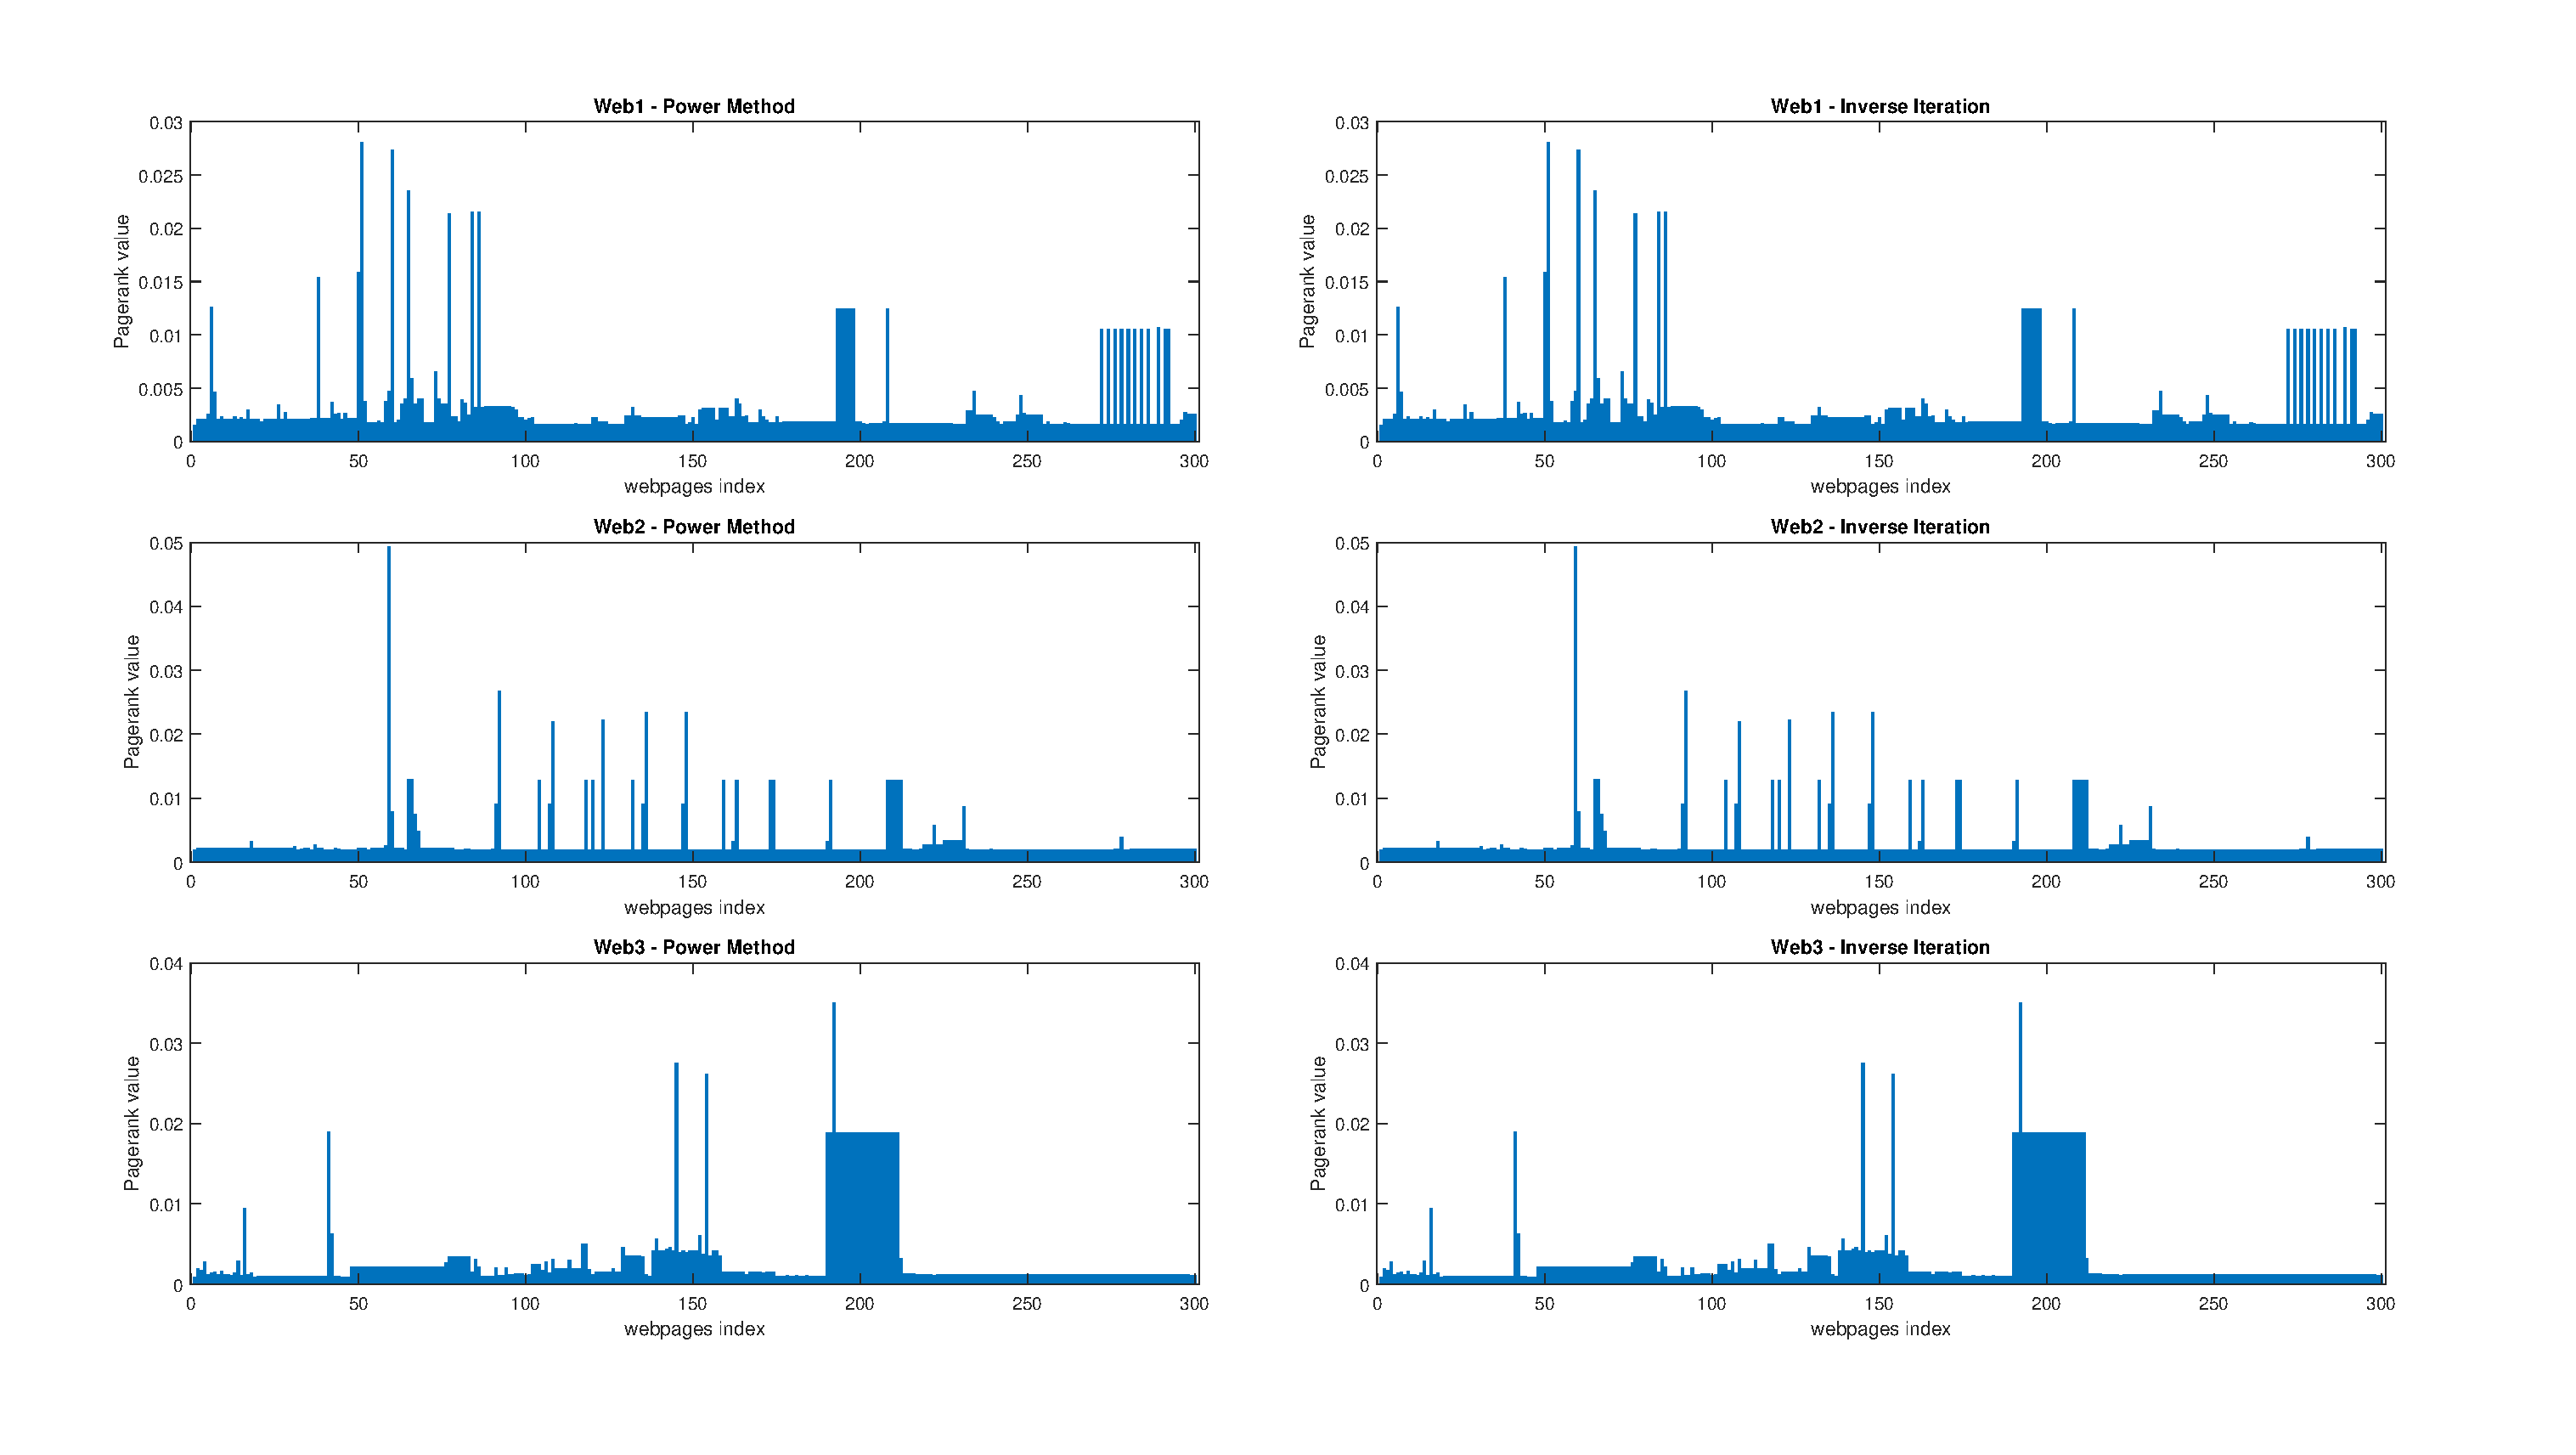
\includegraphics[width=1.2\textwidth, trim={7cm 0 0 0}]{figures/ex4p4_plot.eps}
    \caption{Web1, Web2, Web3 plots from power and inverse iteration methods}
    \label{fig:e4p4_plot}
\end{figure}

\begin{table}[H]
    \centering
    \begin{tabular}{||ccccc||}
        \hline

        \multicolumn{1}{|c|}{\multirow{2}{*}{/}}
             & \multicolumn{2}{l|}{Power Method} & \multicolumn{2}{l|}{Inverse Iteration}              \\ [0.5ex] \cline{2-5}

        \multicolumn{1}{|c|}{}
             & \multicolumn{1}{|c|}{Time avg}    & \multicolumn{1}{|c|}{Iterations}
             & \multicolumn{1}{|c|}{Time avg}    & \multicolumn{1}{|c|}{Iterations}                    \\

        \hline\hline

        Web1 & 8.1237e-04                        & 80                                     & 0.0061 & 6 \\
        Web2 & 5.8967e-04                        & 66                                     & 0.0050 & 6 \\
        Web3 & 0.0012                            & 83                                     & 0.0062 & 6 \\ [1ex]
        \hline
    \end{tabular}
    \caption{Performance comparison on Web graphs}
    \label{tab:ex4p4_comparison}
\end{table}

Timing average values given by \textit{timeit(f)} function in Matlab. \\
In every case the pagerank computation convergences. \\
The pair of vectors resulting from power method and inverse iteration method
correspond as intended for every webpage graphs. \\

Power Method dominance in time complexity in notable from the data retrieved:
it is quick in computing the pageranks and thus giving back the result. \\
Nevertheless, it always performing worser regarding the number of iterations required:
it is always by a magnitude of $10$ greater the number of iterations required
for power method to converge in contrast to inverse iteration which is requiring always $6$ iterations
to achieve the result. \\

Such timing of inverse iteration is due to its complexity to solve linear equation requiring $O(n^3)$
at each iteration and the impossibility of tackle very large graphs without loss in timing.
Thought, inverse iteration method is taking as denoted very few iterations to converge to result
and combined with \textit{Rayleigh Quotient} it reached cubic order of convergence in most cases.
Its application is reserved to special cases and smaller examples where the problem structure enables fast direct methods.


\cleardoublepage

% EXERCISE 5 %%%%%%%%%%%%%%%%%%%%%%%%%%%%%%%%%%%%%%%%%%%%%%%%%%%%%%%%%%%%%%%%%%%%%%%%%%%%%%%%%%%%%%
\subsection{The Reverse Cuthill--McKee Ordering [5 points]}

Load matrix \textit{A\_SymPosDef.mat} from the dataset.
You can reorder (permute) the matrix using "Reverse Cuthill McKee Ordering"
via the Matlab function \textit{symrcm()}, see Matlab documentation for more information.
Visualize both the original and Reverse Cuthill McKee permuted matrix and comment on what you observe.
Compute the Cholesky factor of the original matrix and the permuted matrix.
Visualize the Cholesky factors and comment on the number of nonzeros.

\begin{figure}[H]
    \centering
    \includegraphics{figures/ex5_plot}
    \caption{Matrix A, its R.C.M ordering and their Cholesky factorization}
    \label{fig:ex5_plot}
\end{figure}


Matrix bandwidth: width of the non-zero elements in a matrix, and in our specific case for square matrices
is defined as the maximum distance from a non-zero element to the main diagonal
since upper bandwidth and lower bandwidth correspond.
The computational advantage is given by the fact that band matrices are usually stored
by storing the diagonals in the band; the rest is implicitly zero.\\

The heuristic from the Reverse Cuthill Mckee ordering aims to reduce a matrix bandwidth
by reordering rows and columns. \\
Such reduction decrease significantly the storage and computational work required to handle the matrix. \\
The table shows the difference in bandwidth and consequent computational advantage in timing to compute
the Cholesky decomposition required.

\begin{table}[H]
    \centering
    \begin{tabular}{||c c c||}
        \hline
        Matrix    & Bandwidth & Cholesky avg timing \\ [0.5ex]
        \hline\hline
        A         & 10493     & 1.1592              \\
        symrcm(A) & 234       & 0.0254              \\ [1ex]
        \hline
    \end{tabular}
    \caption{Performance comparison A and its RCM ordering in computing Cholesky factorization}
    \label{table:ex5_cholesky_performance}
\end{table}

Timing average values given by \textit{timeit(f)} function in Matlab. \\
Clearly, given the sparsity of the matrix, computing the Cholesky factorization of matrix $A$
after performing the Reverse Cuthill Mckee ordering magnitudinally increases performance by order
of a hundred in the given case.

\cleardoublepage

% EXERCISE 6 %%%%%%%%%%%%%%%%%%%%%%%%%%%%%%%%%%%%%%%%%%%%%%%%%%%%%%%%%%%%%%%%%%%%%%%%%%%%%%%%%%%%%%
\subsection{Sparse Matrix Factorization [10 points]}

\subsubsection{Construct matrix A for the case n = 10 and explicitly write down its entries. How many non-zero elements does it have?}

\begin{equation} \label{ex6-matrixA}
    A \in \mathbb{R}^{n \times n}, A =
    \begin{bmatrix}
        10 & 1  & 1  & 1  & 1  & 1  & 1  & 1  & 1  & 1  \\
        1  & 11 & 0  & 0  & 0  & 0  & 0  & 0  & 0  & 1  \\
        1  & 0  & 12 & 0  & 0  & 0  & 0  & 0  & 0  & 1  \\
        1  & 0  & 0  & 13 & 0  & 0  & 0  & 0  & 0  & 1  \\
        1  & 0  & 0  & 0  & 14 & 0  & 0  & 0  & 0  & 1  \\
        1  & 0  & 0  & 0  & 0  & 15 & 0  & 0  & 0  & 1  \\
        1  & 0  & 0  & 0  & 0  & 0  & 16 & 0  & 0  & 1  \\
        1  & 0  & 0  & 0  & 0  & 0  & 0  & 17 & 0  & 1  \\
        1  & 0  & 0  & 0  & 0  & 0  & 0  & 0  & 18 & 1  \\
        1  & 1  & 1  & 1  & 1  & 1  & 1  & 1  & 1  & 19 \\
    \end{bmatrix}
\end{equation}

It has $100$ elements: $56$ zero elements and $44$ non-zero elements

\subsubsection{We now want to derive a general formula to compute the number of non-zero entries.
    Show that, for a given matrix $A \in \mathbb{R}^{n \times n}$ with this structure,
    the number of non-zero elements is $5n - 6$.}

There are $5$ elements in set $S = \{top\_row, bottom\_row, left\_column, right\_column, diagonal\}$. \\
Since every element of such set in a square matrix is made of $n$ entries:
$5n$ non-zero entries. \\
Subtract duplicate entries from matrix corners: just $2$ elements of $S$ cover all corners.
Hence subtract every corner extra pair: $2 * 3 = 6$. \\
Finally, there are $5n - 6$ non-zero entries, except for $n = 1$, $A \in \mathbb{R}^{1 \times 1}$ where $nz = 0$.

\begin{equation} \label{eq1}
    \begin{split}
        nz  & = n \cdot |S| - 2 \cdot (|S| - 2) \\
        & = n \cdot 5 - 2 \cdot (5 - 2) \\
        & = 5n - 2 \cdot 3 \\
        & = 5n - 6
    \end{split}
\end{equation}

\subsubsection{Write a function \textit{A\_construct()}, which takes as input $n$ and returns,
    as output, the matrix $A$ akin to matrix \ref{ex6-matrixA} and its number of non-zero elements $nz$.
    Test your function in a script \textit{ex2c.m} for $n = 10$ and compare your results
    with those you obtained in point (1).
    Furthermore, within the same script, visualise the non-zero structure of matrix A by using the command spy()}

\begin{figure}[H]
    \centering
    \includegraphics[width=0.45\textwidth]{figures/ex6p3_spy}
    \caption{Visualization spy() of matrix $A$}
    \label{fig:ex6p3_spy}
\end{figure}

The function correctly computes matrix A with 44 non-zero elements.
The script containing further visualization of the matrix on the terminal and
double checks the non-zero elements correctness.

\subsubsection{Using again the \textit{spy()} command, visualize side by side
    the original matrix $A$ and the result of the Cholesky factorization (\textit{chol()} in Matlab).}

\begin{figure}[H]
    \centering
    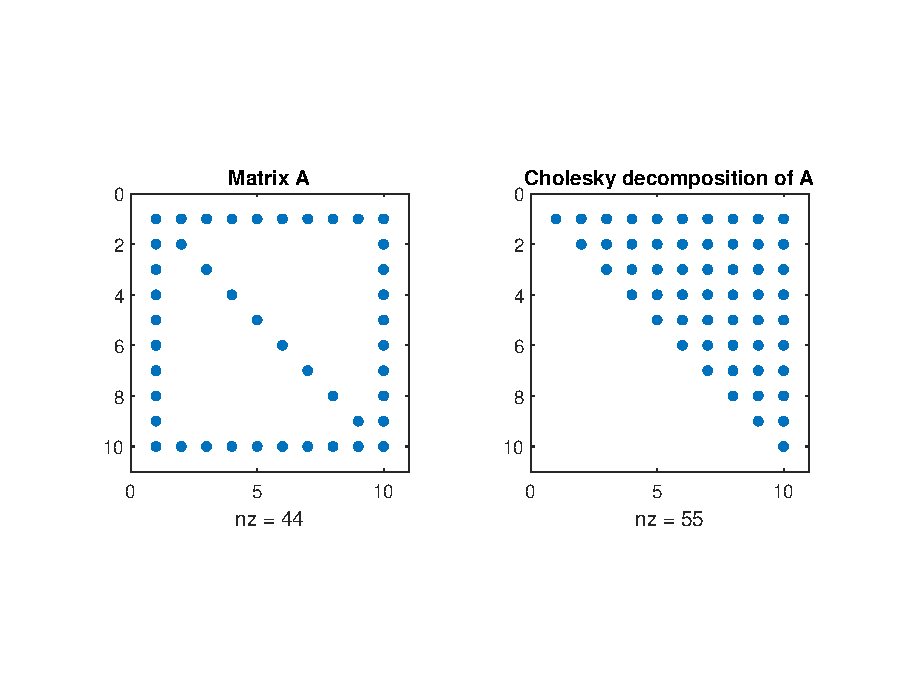
\includegraphics[width=0.7\textwidth]{figures/ex6p4_spy}
    \caption{Visualization of $A$ and its Cholesky factorization}
    \label{fig:ex6p4_spy}
\end{figure}

\subsubsection{Explain why, for $n = 100\,000$, using \textit{chol()} to solve $Ax = b$
    for a given right-hand-side vector $b$ would be problematic.
    Are there ways to mitigate this issue?}

Cholesky decomposition needs to solve linear equations, each of them requiring $O(n^3)$ time complexity. \\
Having set $n = 100\,000$ makes the problem unbearable.
An analogy is the example of why inverse iteration is not used for Internet ranking:
solving linear equation of very large $n$ is discouraged. \\
Without setting matrix $A$ to be sparse, Matlab promptly yields: \\

\textit{Requested 100000x100000 (74.5GB)
    array exceeds maximum array size preference (15.7GB).
    This might cause MATLAB to become unresponsive.} \\

Initializing the matrix with sparse, it tries to compute it but after a while
an evident great amount of time will be required with such $n$.  \\

A way to mitigate this could be to permutate the matrix using the previous
Reverse Cuthill Mckee ordering so the computation complexity decreases magnitudinally
becoming feasable for relatively large $n$.

\cleardoublepage

% EXERCISE 7 %%%%%%%%%%%%%%%%%%%%%%%%%%%%%%%%%%%%%%%%%%%%%%%%%%%%%%%%%%%%%%%%%%%%%%%%%%%%%%%%%%%%%%
\subsection{Degree Centrality [5 points]}

In graph theory and network analysis, centrality refers to indicators which identify
the most important vertices within a graph.
Applications include identifying the most influential person(s) in a social network,
key infrastructure nodes in the Internet or urban networks, and super spreaders of disease.
Here we are interested in the \textbf{Degree centrality}, which is conceptually simple.
It is defined as the number of links incident upon a node
(i.e., the number of vertices that a node has).
The degree centrality of a vertex $v$, for a given graph
$G := (V, E)$ with $|V|$ vertices and $|E|$ edges, is defined as the numbers of edges of vertex $v$. \\
Compute the degree centrality for the top 5 authors.
Include them in an ordered list, and show the authors, the their coauthors and the degree centrality. \\

\begin{table}[H]
    \centering
    \begin{tabular}{||c c p{5in}||}
        \hline
        Author    & Degree & Coauthors                                                                                                                                                                                                                                                          \\ [0.5ex]
        \hline\hline
        Golub     & 33     & Wilkinson, TChan, Varah, Overton, Ernst, VanLoan, Saunders, Bojanczyk, Dubrulle, George, Nachtigal, Kahan, Varga, Kagstrom, Widlund, OLeary, Bjorck, Eisenstat, Zha, VanDooren, Tang, Reichel, Luk, Fischer, Gutknecht, Heath, Plemmons, Berry, Sameh, Meyer, Gill \\ \hline
        Demmel    & 17     & Edelman, VanLoan, Bai, Schreiber, Kahan, Kagstrom, Barlow, NHigham, Arioli, Duff, Hammarling, Bunch, Heath, Greenbaum, Gragg                                                                                                                                       \\ \hline
        Plemmons  & 15     & Golub, Nagy, Harrod, Pan, Funderlic, Bojanczyk, George, Barlow, Heath, Berry, Sameh, Meyer, Nichols                                                                                                                                                                \\ \hline
        Schreiber & 14     & TChan, VanLoan, Moler, Gilbert, Pothen, NTrefethen, Bjorstad, NHigham, Eisenstat, Tang, Elden, Demmel                                                                                                                                                              \\ \hline
        Heath     & 14     & Golub, TChan, Funderlic, George, Gilbert, Eisenstat, Ng, Liu, Laub, Plemmons, Paige, Demmel                                                                                                                                                                        \\ [1ex]
        \hline
    \end{tabular}
    \caption{top 5 authors ordered with their degree and coauthors}
    \label{table:ex7_top5authors}
\end{table}

The degree in Matlab is given by $degree(graph(A), node_num)$.
Number of coauthors for each author is degree of author $-2$ to remove the double self reference: one in and one out of the same node.
It does not change the result of the ordered list.\\

\cleardoublepage

% EXERCISE 8 %%%%%%%%%%%%%%%%%%%%%%%%%%%%%%%%%%%%%%%%%%%%%%%%%%%%%%%%%%%%%%%%%%%%%%%%%%%%%%%%%%%%%%
\subsection{The Connectivity of the Coauthors [5 points]}

How many coauthors have the authors in common?
Think about a general procedure that allows you to compute the list of common coauthors of two authors
and express it in matrix notation.
Use the formula you derived to compute the common coauthors of the pairs
(Golub, Moler), (Golub, Saunders), and (TChan, Demmel).
Who are these common coauthors? Report their names. \\

Every column from adjacency matrix $A$ is relative to an author:
it contains all the coauthors any author $a_1$ has collaborated with. \\
For any other author $a_2$, to find common coauthors between $a_1$ and $a_2$ just compare column entries looking for edges in correspondent indexes
excluding the same $a_1$, $a_2$ from result. \\

\begin{gather*} \label{ex8_common_coauthors}
    A \in \mathbb{R}^{n \times n} \nonumber\\
    a_i, a_j \in S = \{\text{authors}\},\ n = |S| \nonumber\\
    \text{columns } \myv{c}',\ \myv{c}'':\ \myv{c}' = A_{l a_i},\ \myv{c}'' = A_{l a_j}, l \in {1, \dots, n} \nonumber\\
    u_k \in S' = \{\text{common coauthors}\} \nonumber\\
    u_k = \begin{cases}
        1 & if\ \myv{c}_k' = 1 \land \myv{c}_k'' = 1 \land k \neq i \land k \neq j \nonumber \\
        0 & otherwise
    \end{cases} \nonumber\\
    \begin{split}
        S'  &= A_{l a_1} \cap A_{l a_2},\, l \in {1, \dots, n} \nonumber\\
        &= c' \cap c''
    \end{split}
\end{gather*}

From Matlab script implementation of exercise \textit{ex8.m}:

\begin{table}[H]
    \centering
    \begin{tabular}{||l l||}
        \hline
        Pair              & Common Coauthors               \\ [0.5ex]
        \hline\hline
        (Golub, Moler)    & Wilkinson, VanLoan             \\
        (Golub, Saunders) & Gill                           \\
        (TChan, Demmel)   & Schreiber, Arioli, Duff, Heath \\[1ex]
        \hline
    \end{tabular}
    \caption{Common coauthors of pairs}
    \label{table:ex8_common_coauthors}
\end{table}

\cleardoublepage

% EXERCISE 9 %%%%%%%%%%%%%%%%%%%%%%%%%%%%%%%%%%%%%%%%%%%%%%%%%%%%%%%%%%%%%%%%%%%%%%%%%%%%%%%%%%%%%%
\subsection{PageRank of the Coauthor Graph [5 points]}

Compute the PageRank value (e.g., by using a modified version of \textit{pagerank.m}
from Project 1) for all authors and provide a graph of all authors in descending order
according to the PageRank.
Include your script in the submission. \\

\begin{figure}[H]
    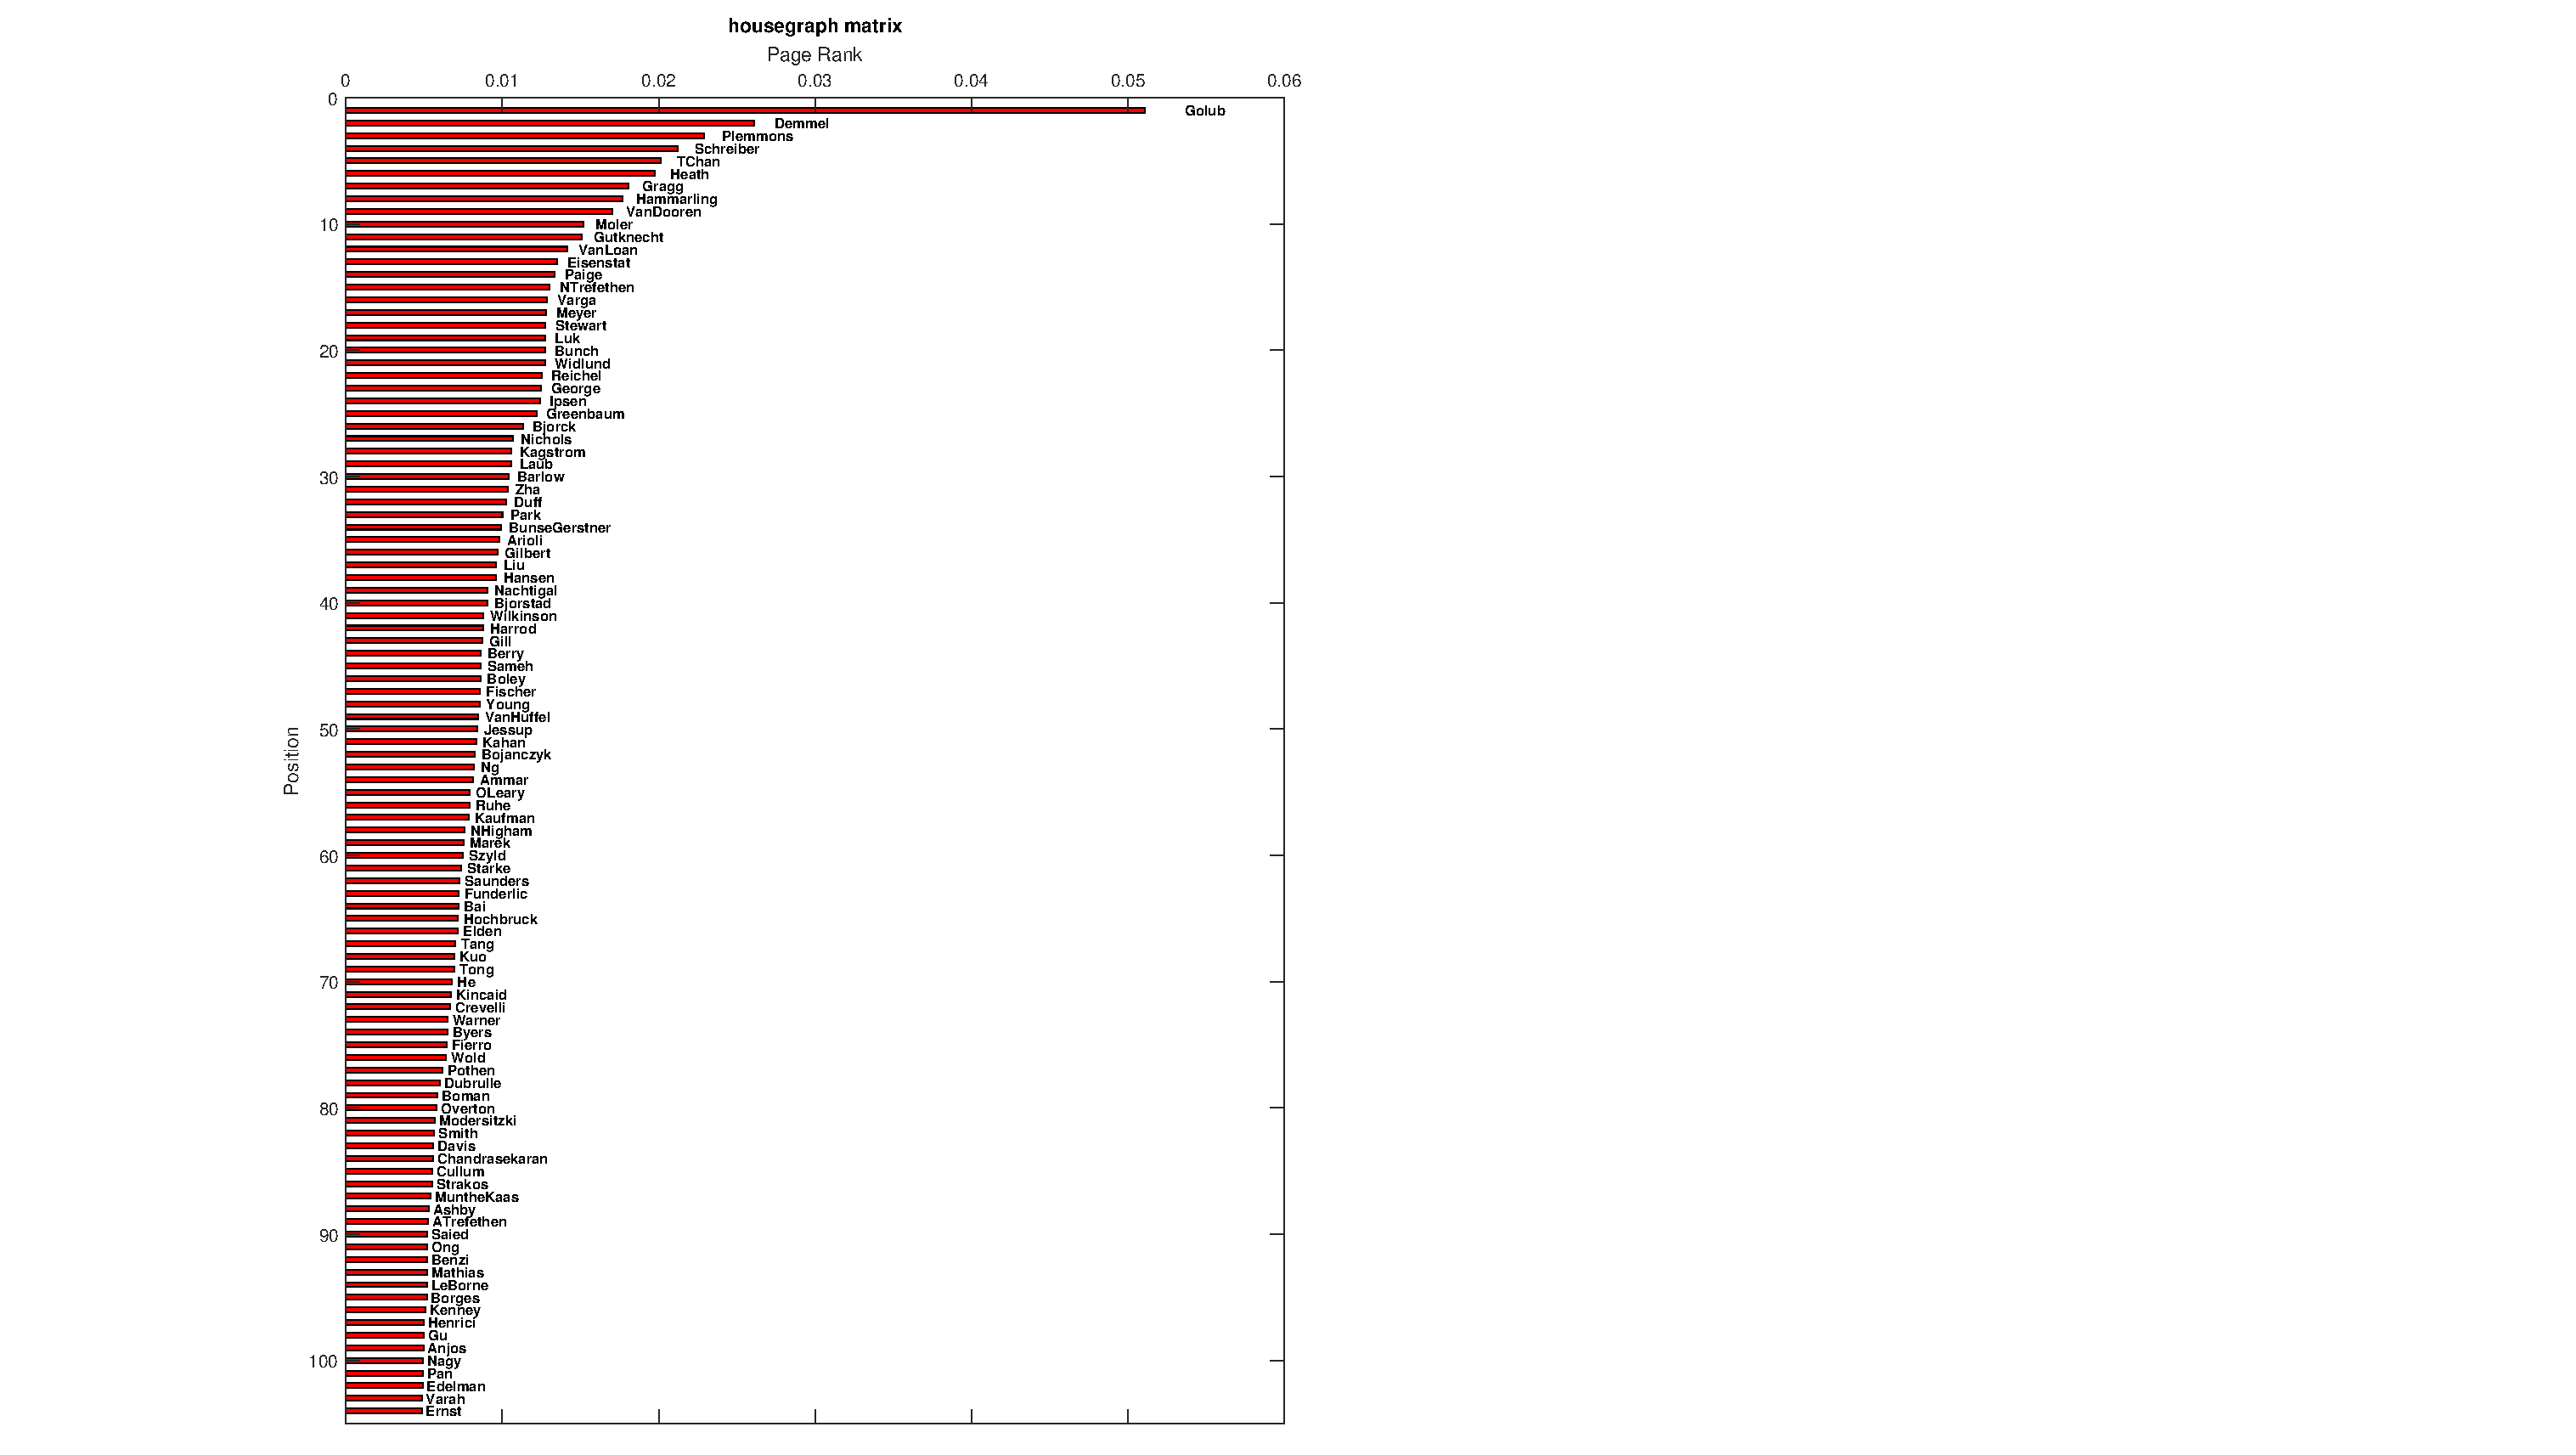
\includegraphics[width=2\textwidth, trim={5cm 0 0 0}]{figures/ex9_pagerank}
    \caption{Pagerank of Housegraph}
    \label{fig:ex9_pagerank}
\end{figure}

This histogram emphasize the concept of $Degree \neq PageRank$.

\end{document}
